\documentclass{documentation}
\usepackage{graphicx}
\showhelp  % comenta o borra para eliminar ayudas

\selectlanguage{spanish}

%TITLE
\title{wearControl}
\author{Josue Gutierrez Duran}
\advisorFirst{\url{https://github.com/JoxuMac/wearControl}}
\docdate{2017}{Diciembre}
\begin{document}

\maketitle
\tableofcontents

\newpage

\section{DESCRIPCIÓN GENERAL}


Los smartwatch son dispositivos electrónicos inteligentes que están claramente en auge. Gracias a ellos es posible extender funciones de los dispositivos móviles u ordenadores. Dado que en la asignatura de referencia \textit{Multimedia} se han tratado temas referentes a Audio y Vídeo. Se propone realizar una aplicación wear que sea capaz de controlar los controles multimedia de un ordenador. Esta aplicación sera independiente de un dispositivo móvil, no siendo necesario este para funcionar. Por lo que sera necesario que el smartwatch tenga conexión Wi-Fi. 
\newline
\par
\noindent
Para la realización de este proyecto se desarrollaran dos aplicaciones distintas, una primera aplicación que se ejecutara en el ordenador que se desea controlar, y una segunda aplicación ejecutada en el smartwatch que actuara como mando a distancia.

\section{REQUISITOS DE LA APLICACIÓN}

Para este trabajo, se deben de cumplir algunos de los requisitos propuestos en la documentación de la asignatura y adjuntados en el \textbf{Cuadro 1}. Por tanto, se proponen los requisitos de aplicación registrados en el \textbf{Cuadro 2}.

\begin{table}[hp]
  \centering
  \caption{Requisitos Generales del Trabajo}
  \label{tab:tec-especifica}

  \zebrarows{1}
  \begin{tabular}{p{0.6\textwidth}}
    \hline
    Comunicación \\
    Descarga, actualización \\
    Visualización y/o reproducción \\
    Interacción con usuario y/o con otros sistemas Hw/Sw \\
    Compresión \\
    Procesamiento de señales \\
    \hline
  \end{tabular}
\end{table}


\begin{table}[hp]
  \centering
  \caption{Requisitos de la Aplicación wearControl}
  \label{tab:competencias}

  \zebrarows{1}
  \begin{tabular}{p{1\textwidth}}
    \hline
    La aplicación wear debe de ser independiente de cualquier otro dispositivo\\
    La conexión entre PC y Android Wear debe de ser a traves de una red Wi-Fi\\
    Deben de poderse conectar mas de un sistema en una misma red local\\
    Debe de ser posible controlar desde el smartwatch los controles multimedia, tales como Play, Stop, Back y Next.\\
    Debe de ser posible controlar los controles de Volumen; Up, Down y Mute. \\
    Debe de ser posible abrir aplicaciones multimedia en el PC, Spotify, VLC y iTunes \\
    \hline
  \end{tabular}
\end{table}

\newpage
\section{DECISIONES Y JUSTIFICACIÓN DE DISEÑO E IMPLEMENTACIÓN}

Como protocolo de comunicación utilizaremos UDP, ya que este no es orientado a conexión y así no sera necesario introducir direcciones IPs en ninguno de los dos dispositivos.
\newline
\par
\noindent
Realizaremos un Broadcast desde el equipo de escritorio, ya que por limitaciones de Hw/Sw, no es posible realizarlo desde el smartwatch. El Broadcast realizado por el PC enviara su código PIN por la red local cada 15 segundos. Al mismo tiempo, pondrá otro hilo a la escucha, a la espera de un mensaje compuesto del código PIN '-' y la orden a ejecutar en código binario (Ej. 1234-0000). Si el código PIN no corresponde con el configurado en la aplicación, esta desechara dicho mensaje.
\newline
\par
\noindent
La aplicación SmartWatch, tendrá un hilo a la escucha, esperando el mensaje Broadcast que envía la aplicación de escritorio. Una vez le llegue este mensaje y compruebe que el PIN enviado, corresponde con el configurado en el reloj, almacena dicha IP. Por otro lado, siempre que se pulse un botón en el reloj, se enviara un mensaje a la IP almacenada con el formato anterior (PIN-ORDEN)


\section{CONCLUSIONES}

Como conclusión, gracias al desarrollo de este proyecto, hemos podido aprender la importancia y protocolos de comunicación y paso de mensajes. Ademas, gracias a la implementación de la aplicación wear, es importante tener en cuenta la interacción con el usuario ya que esta debe de ser intuitiva y ligera. 

Se ha indagado sobre como manejar la reproducción de los controles multimedia de un ordenador, tales como volumen o media en diferentes lenguajes, tales como JAVA, C\# y VB

Ademas, gracias al uso de un repositorio, se ha afianzado el conocimiento y uso del mismo.
\newpage
\section{BIBLIOGRAFÍA}

Como Bibliografía utilizada en este trabajo, tenemos diferentes paginas web y documentación referente al diseño de aplicaciones Android Wear, a continuación se nombran todas las referencias utilizadas.

\begin{itemize}
\item Android Web Developers - \url{https://developer.android.com}
\item Smartwatch Tutorial - Android Wear for Beginners - \url{http://www.smartwatch.me/t/tutorial-how-to-develop-android-wear-apps-for-beginners-part-1-setup/684}
\item StackOverFlow - \url{https://stackoverflow.com/}
\end{itemize}


\section{MANUAL DE USUARIO}

Para que wearControl funcione, el smartwatch y el ordenador deben de estar conectados en la misma red local, y que esta permita la inundación Broadcast en la red por el protocolo UDP.

\subsection{PC}

Una vez instalada la aplicación .exe en su ordenador, ejecútela.

En la barra de Tareas, aparecerá el icono de la aplicación wearControl.
\begin{figure}[!ht]
	\centering
	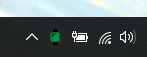
\includegraphics[width=0.5\textwidth]{figures/pc/1.png}
	\caption{Barra de Tareas}
\end{figure}
\newpage
Haciendo click derecho sobre el icono, nos aparecerá la opción de 'Salir' o de 'Configuración' para poder configurar los parámetros de la aplicación de escritorio

\begin{figure}[!ht]
	\centering
	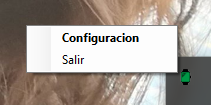
\includegraphics[width=0.5\textwidth]{figures/pc/2.png}
	\caption{wearControl}
\end{figure}

En la ventana de configuracion, podremos cambiar el numero PIN, cambiar el idioma a 'Español' o a 'Ingles' y especificar la ruta de las aplicaciones que podremos abrir con el SmartWatch; 'VLC', 'Spotify' o 'iTunes'.

\begin{figure}[!ht]
	\centering
	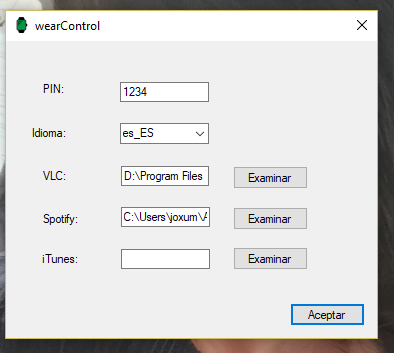
\includegraphics[width=0.5\textwidth]{figures/pc/3.png}
	\caption{Ventana de Configuración}
\end{figure}

\newpage
\subsection{SmartWatch}

Una vez instalada la aplicación .apk en su dispositivo wear, ábrala teniendo abierta la aplicación de escritorio en su ordenador.

En la primera pantalla podrá enviar las ordenes de 'PLAY/PAUSA' para Reproducir o Pausar un contenido, 'PREVIOUS' para retroceder, 'NEXT' para Avanzar y 'STOP' para parar la reproducción.

\begin{figure}[!ht]
	\centering
	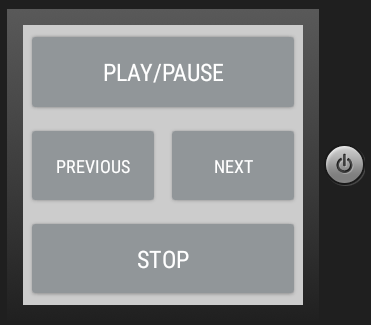
\includegraphics[width=0.5\textwidth]{figures/sw/1.png}
	\caption{Pantalla 1}
\end{figure}

Si deslizamos la pantalla de derecha a izquierda, cambiaremos a los controles del sonido; 'VOL +' para subir el volumen de nuestro ordenador, 'VOL -' para bajarlo y 'MUTE/UNMUTE' para poner y quitarle el sonido.

\begin{figure}[!ht]
	\centering
	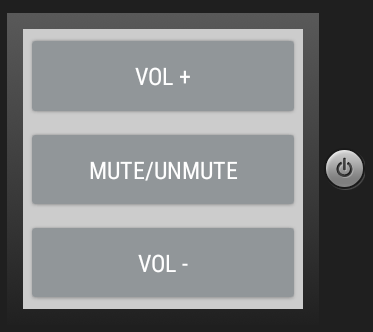
\includegraphics[width=0.5\textwidth]{figures/sw/2.png}
	\caption{Pantalla 2}
\end{figure}

Deslizando una tercera vez de derecha a izquierda, tendremos un menú en el que se nos proponen varias opciones, pudiendo elegir entre 'Applications' para poder abrir aplicaciones, 'Configuration' para entrar en los ajustes de la aplicación wear y 'Credits' para acceder a los créditos del proyecto.

\begin{figure}[!ht]
	\centering
	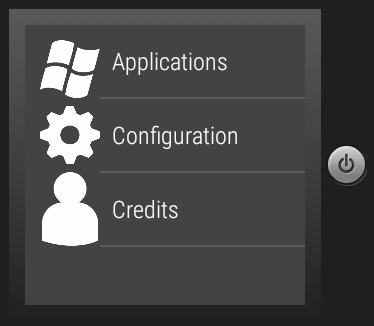
\includegraphics[width=0.5\textwidth]{figures/sw/3.png}
	\caption{Pantalla 3}
\end{figure}

Abriendo el menú 'Applications' podremos abrir diferentes aplicaciones en nuestro ordenador (Siempre que estén configuradas en la aplicación de escritorio), tales como 'VLC', 'Spotify' y 'iTunes'

\begin{figure}[!ht]
	\centering
	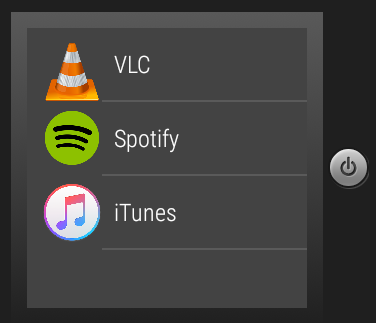
\includegraphics[width=0.5\textwidth]{figures/sw/4.png}
	\caption{Pantalla Aplicaciones}
\end{figure}
\newpage
En el menú de 'Configuration' podemos elegir el código PIN deseado, debemos de tener en cuenta de que debe de ser el mismo código PIN que el de la aplicación de escritorio.

\begin{figure}[!ht]
	\centering
	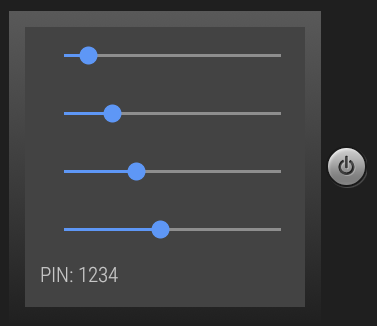
\includegraphics[width=0.5\textwidth]{figures/sw/5.png}
	\caption{Pantalla Configuración}
\end{figure}

Desde el menú de 'Credits' podremos observar la información respectiva del proyecto; Nombre, Version, Desarrollador y Asignatura

\begin{figure}[!ht]
	\centering
	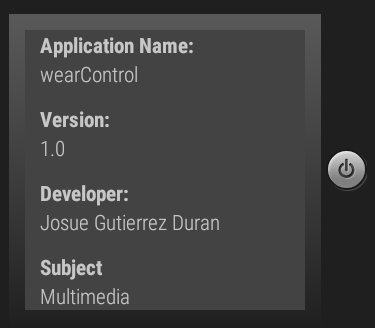
\includegraphics[width=0.5\textwidth]{figures/sw/6.png}
	\caption{Pantalla Créditos}
\end{figure}



\end{document}


% Local Variables:
% coding: utf-8
% mode: flyspell
% ispell-local-dictionary: "castellano8"
% mode: latex
% End:
